\chapter{Correlative Analysis}

Purpose:

-briefly introduce why I think correlative analysis is valuable
-talk about some basic correlative theory and statistic analysis
-lay out various correlation score techniques
-talk about their limitations and some alternatives
-choose what I think is most appropriate for this problem
--lay out argument for PCC, perhaps

We borrowed insight and several visualization techniques from the literature. Cancro et al. developed useful techniques for packing large numbers of channels into a dense rectangular space \cite{Cancro}, and Yairi et al. demonstrated ways to show change correlation between data channels \cite{Yairi}, which were inspirations for our Global Correlation Matrix and Channel Correlation Vector. 


\section{Correlation for Fault Analysis}

\subsection{Correlation Matrices}



\subsection{Cross-Correlative Leak Analysis}

Isermann paper

Discussion of how this is using correlation between telemetry values to look for an understood fault state, rather than for data discovery (but it's still valuable!)

\section{Common Correlation ``Score" Techniques}

When looking at two sets of data, it can often be valuable to reduce their interdependence (i.e., how much they change in sync with each other) into a single number, or ``correlation coefficient." This coefficient can be used as straightforward metric to determine correlation between sets of times series data. It may even be used as input into visualization algorithms to affect shading or even positioning, as we will see in later chapters.

\subsection{Pearson Correlation Coefficient}

The Pearson Correlation Coefficient (PCC), also known as the Pearson Product-Moment Coefficient, is a metric of the linear relationship between two sets of data. It is essentially a scaled covariance, defined as \\

\begin{equation} \label{eq:pcc}
\rho_{X, Y} = \frac{\mathrm{cov}(X, Y)}{\sigma_{X} \sigma_{Y}}
\end{equation}

where $X$ and $Y$ are two vectors of data (or, in the case of the telemetry data sets we examine in this paper, times series of values over time for two telemetry channels). The PCC gives a quantified measurement of the linear correlation between the two vectors, in the form of a value in the range of $[-1, 1]$, where $1$ is a total positive correlation, $-1$ is a total negative correlation, and $0$ is no correlation at all.

The Pearson Correlation Coefficient carries with it a few important assumptions:

\begin{itemize}
\item Samples have values that are interval or ratio variables (not ordinal or categorical)
\item Sample pairs follow a bivariate normal distribution
\item Sample pairs have a linear relationship (or, at least, these are the type of relationships you wish to see)
\end{itemize}

If the data doesn't fit the assumptions above, one of the two rank correlation coefficients discussed below may be more appropriate.

\subsection{Spearman Rank Correlation Coefficient ($\rho$)}

The Spearman Rank Correlation Coefficient, or Spearman's rho, is a type of correlation coefficient, which, like the PCC, seeks to quantify relationships between vectors of data, but which looks the ranking of variables within an ordering, rather than their linear relationship. This allows the coefficient to express relationship \textit{monotonicity}, in order to be less dependent on linearity of relationships. It actually makes uses of the PCC to do this, by calculating the PCC on the ranked data values.

\subsection{Kendall Rank Correlation Coefficient ($\tau$)}

The Kendall Rank Correlation Coefficient, like Spearman's rho, seeks to capture non-linear dependence by using the ordered ranks of the argument variables as input to the algorithm.

A visual comparison of the Pearson Correlation Coefficient, Spearman Rank Correlation Coefficient, and Kendall Rank Correlation Coefficient is shown in Fig.~\ref{fig:correlation_comparison}.

\begin{figure}[h]
\centering
    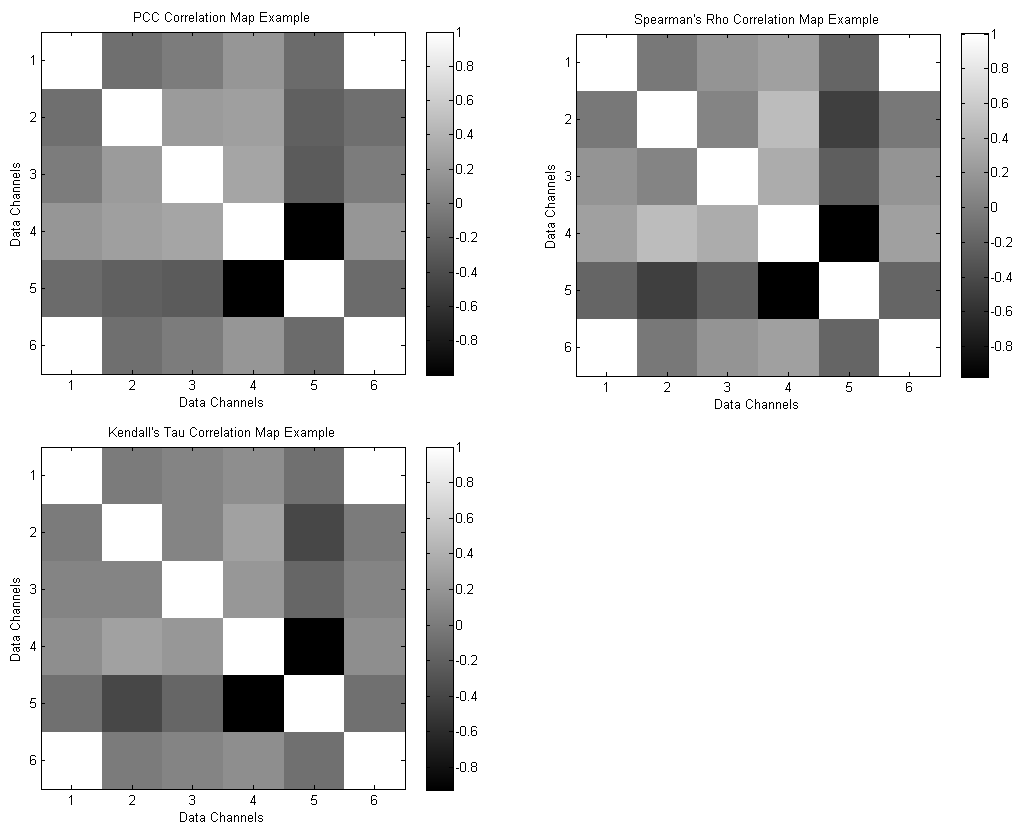
\includegraphics[width=\columnwidth]{images/correlation_comparison.png}
    \caption{Three common correlation coefficient algorithms are compared on a sample data set. Note that 1 and 6 have a strong rank-based correlation, but the relationship is non-linear, resulting in a visibly lower correlation score within the PCC visualization. Also note the strong negative correlation between items 4 and 5.}
    \label{fig:correlation_comparison}
\end{figure}





\section{Limitations of Traditional Correlative Techniques}

There are many limitations to the three traditional correlative techniques above, and it's important to understand them, even if the ultimate decision will be to use one of these techniques. Some of the major limitations are decribed below.

\subsection{Linearity Assumptions}

The PCC algorithm, in particular

In contrast, the rank correlation methods 

\subsection{Multivariate Normal Distances vs. Elliptical Distances}

\subsection{Implied Causation}

\subsection{Alternatives to Correlation Score Techniques}



\subsection{Distance Correlation}

\subsection{Correlation Ratio}

\subsection{Brownian Covariance}

\subsection{Coefficient of Determination}

\subsection{Polychloric Correlation}